\section{Introduction to Wazuh}
\subsection{What is Wazuh?}
Wazuh stands as a free and open-source security platform, wielding the combined power of XDR (extended detection and response) and SIEM (security information and event management). This potent combination safeguards data across diverse environments, from traditional on-premise setups to the modern world of cloud, virtual, and containerized systems.

Wazuh builds upon the capabilities of OSSEC (an open-source intrusion detection system), further enhancing its functionality with additional features, richer APIs, and improved integration capabilities. Trusted by organizations of all sizes, Wazuh offers a reliable defense against ever-present security threats.

\subsection{Wazuh Components}
Wazuh primarily comprises of 2 components: the Wazuh Agent and the Wazuh Manager.

\subsubsection{Wazuh Agent}

The Wazuh agent, a multi-platform component, runs on user-designated endpoints for monitoring purposes. It transmits data to the Wazuh server in near real-time via an encrypted and authenticated channel. Designed with performance in mind for diverse endpoints, the agent supports popular operating systems (like Windows, Linux, macOS, Solaris etc.) and requires a modest average of 35 MB RAM.

The Wazuh agent empowers users with a range of security-enhancing features, including:

\begin{itemize}
    \item Log collection
    \item Command execution
    \item File integrity monitoring (FIM)
    \item Security configuration assessment (SCA)
    \item System inventory
    \item Malware detection
    \item Active response
    \item Container security
    \item Cloud security
\end{itemize}


\subsubsection{Wazuh Manager}

The Wazuh Manager, also known as the `Central Component' acts as the core of the Wazuh system. It comprises three key elements:

\begin{enumerate}
    \item \textbf{Wazuh Indexer:} This highly scalable engine serves as a full-text search and analytics platform. It indexes and stores alerts generated by the Wazuh server, enabling efficient retrieval and analysis.

    \item \textbf{Wazuh Server:} Functioning as the data processing center, the Wazuh server analyzes information received from agents. It employs decoders, rules, and threat intelligence to identify potential security breaches based on known indicators of compromise (IOCs). A single server can handle data from hundreds or thousands of agents, with the capability to scale horizontally in a cluster configuration. Additionally, the Wazuh server manages the agents, allowing for remote configuration and upgrades.

    \item \textbf{Wazuh Dashboard:} This web-based user interface provides a platform for data visualization and analysis. Pre-configured dashboards offer insights into security events, regulatory compliance (PCI DSS, GDPR, CIS, HIPAA, NIST 800-53, etc.), detected vulnerabilities, file integrity monitoring data, configuration assessment results, cloud infrastructure events, and more. It also facilitates Wazuh configuration management and status monitoring.
\end{enumerate}

\begin{figure} [H]
\centering
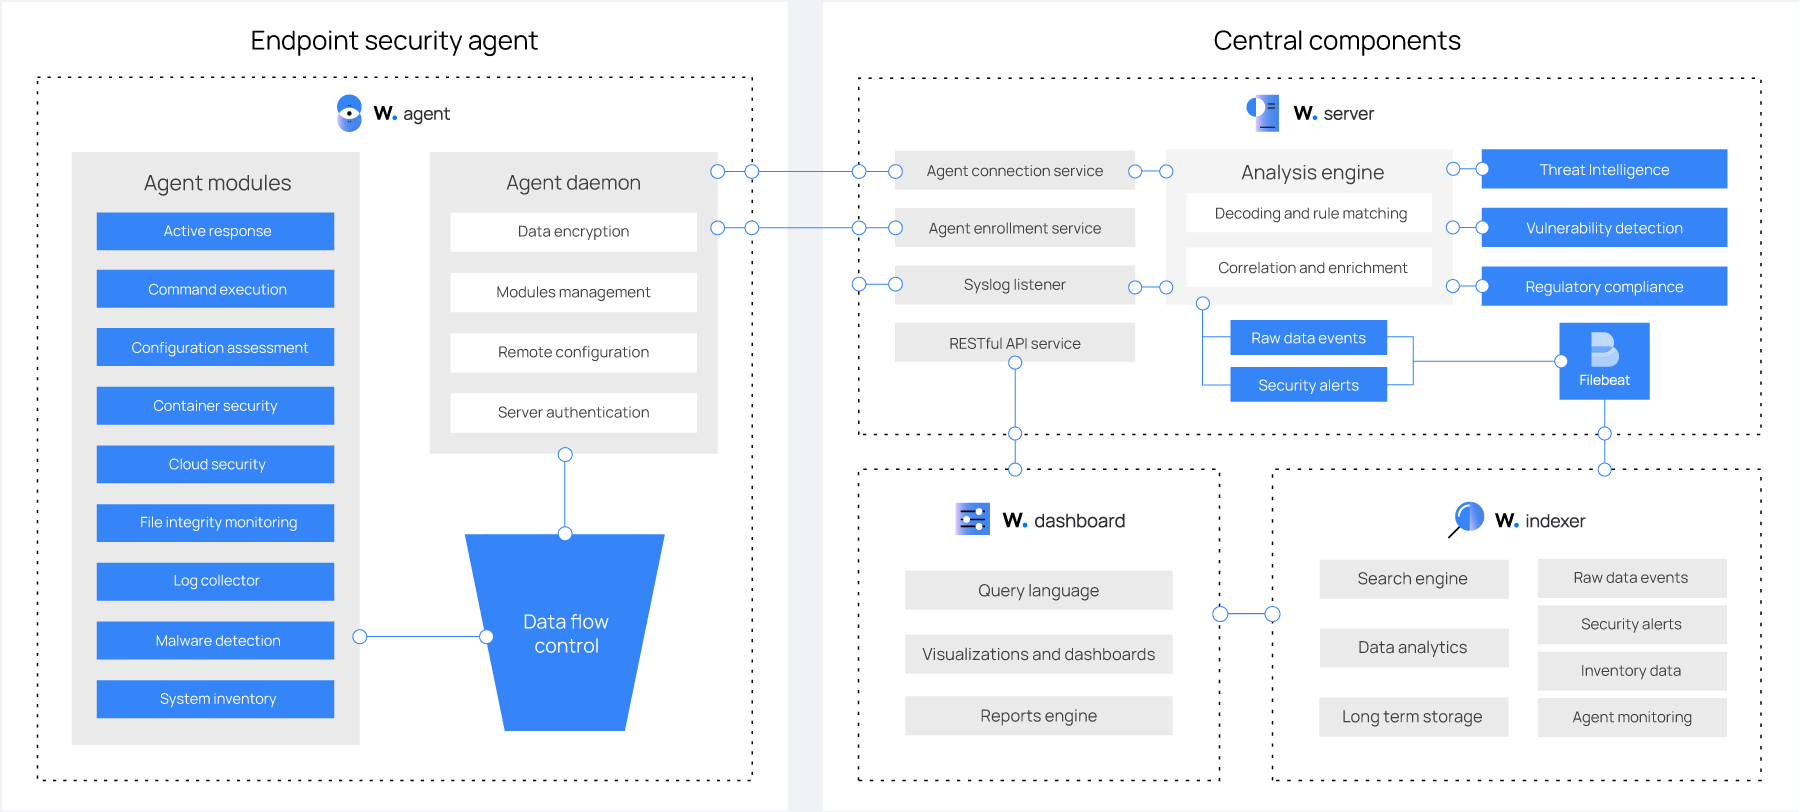
\includegraphics[width=\textwidth]{images/components-data-flow.png}
\caption{Wazuh Components and Data flow}
\label{fig:wazuhcomponents}
\end{figure}

\subsection{Wazuh Architecture}

The foundational structure of the Wazuh system hinges on two primary components: agents and servers. Agents, installed on monitored systems, relay security data back to the centralized server. The system also accommodates agentless devices like firewalls and routers, enabling these to transmit log data through various protocols such as Syslog and SSH, or directly via APIs.

Upon receipt, the central server undertakes the decoding and analysis of this data, thereafter dispatching it to the Wazuh indexer. The indexer, potentially a single-node for smaller setups or a multi-node cluster for larger, data-intensive operations, is tasked with data indexing and preservation.

Particularly in production settings, segregating the server and indexer onto separate platforms enhances system integrity. Within this framework, Filebeat plays a critical role, securely shuttling alerts and archives from the Wazuh server to the indexer, all the while safeguarded by TLS encryption.

Illustrated below, the deployment architecture schema delineates the interplay between server and indexer within the ecosystem, underscoring the potential for cluster configurations to achieve scalability and fault tolerance.

\begin{figure} [H]
\centering
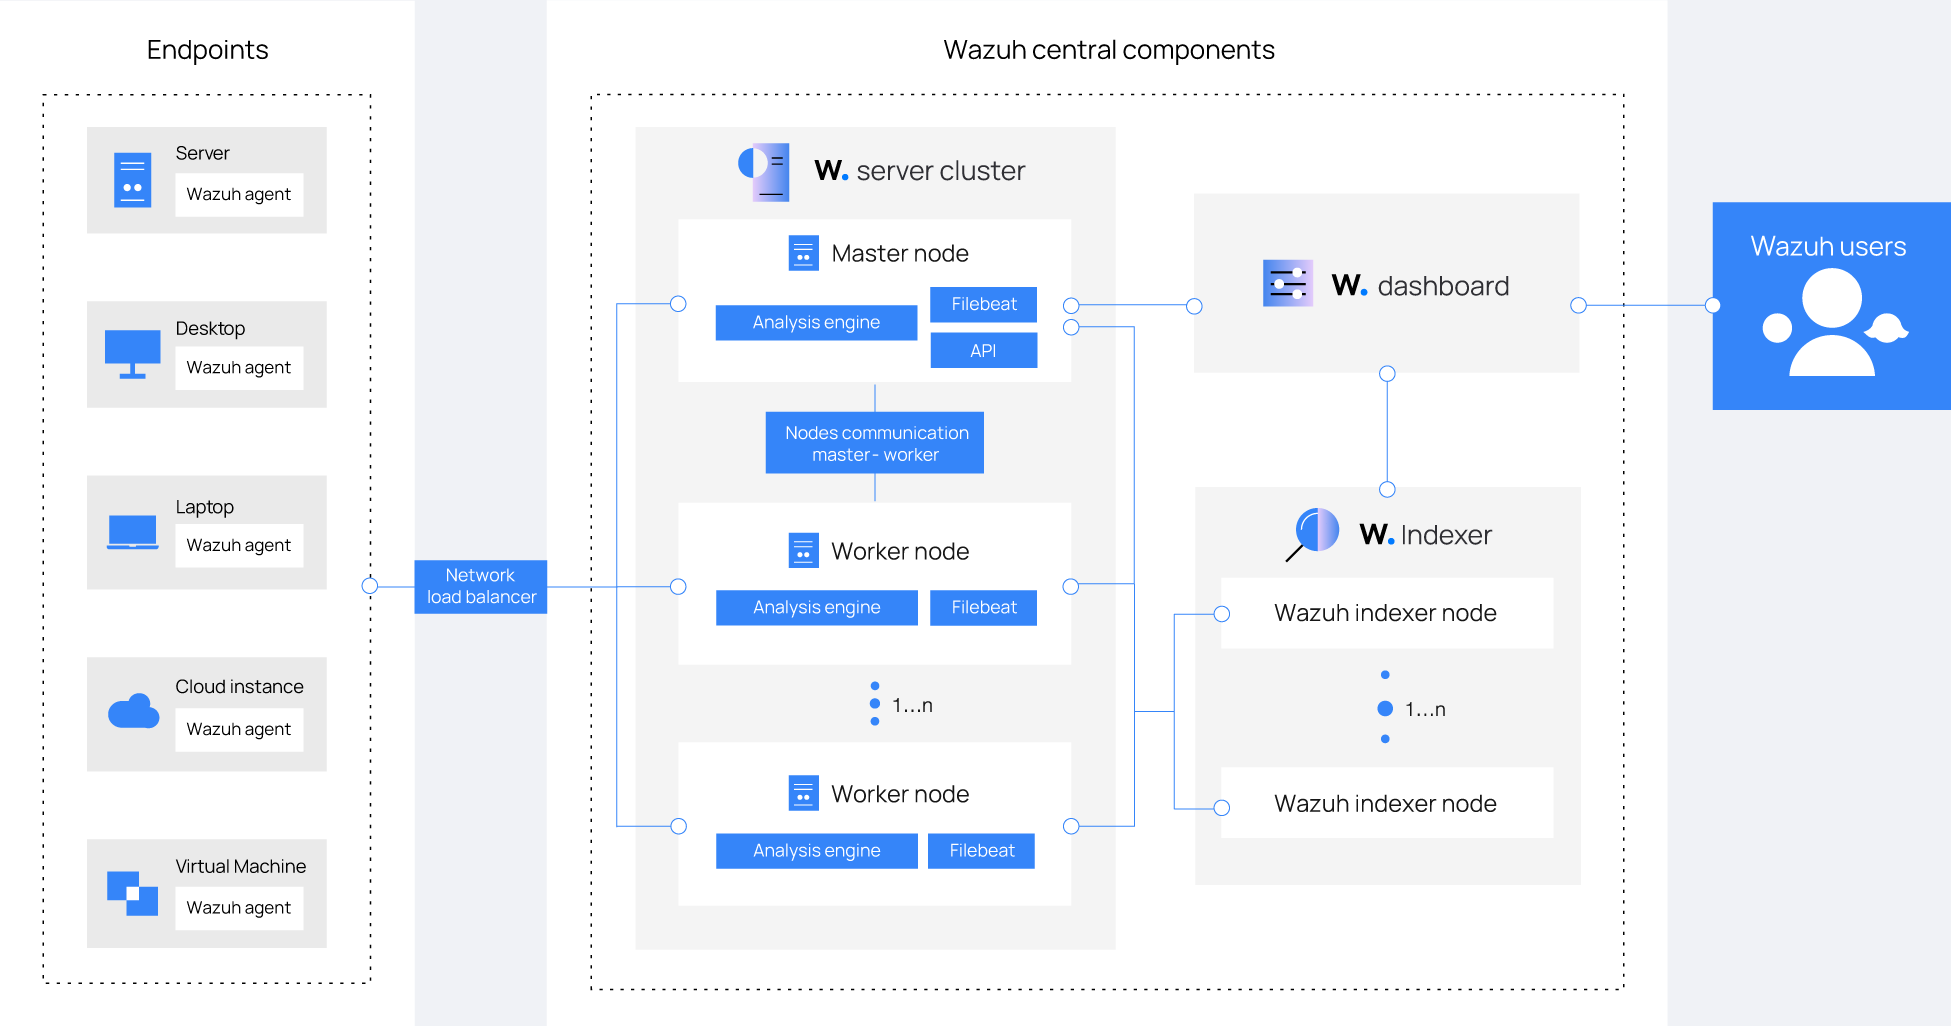
\includegraphics[width=\textwidth]{images/architecture.png}
\caption{Overview of Wazuh Deployment Architecture}
\label{fig:wazuharchitecture}
\end{figure}
